% ====================================================================
%  CHAPTER 1: INTRODUCTION
%  Section headings follow the Makerere MSc proposal structure.
%  Replace the guidance notes and bracketed placeholders with your text.
% ====================================================================
\chapter{INTRODUCTION}\label{ch:1}

\section{Background to the Study}\label{sec:1.1}
\guidance{Move from the general to the specific in three or four paragraphs: the subject and its importance, the constraint or problem, what is already known, and what remains unresolved. Cite as you go.}

{[}Opening paragraph establishing the subject and its importance \parencite{example_2020_article}.]

{[}Second paragraph narrowing to the constraint your study addresses \parencite{example_2019_book, example_2021_chapter}.]

\section{Problem Statement}\label{sec:1.2}
\guidance{One paragraph. State the problem, the evidence that it is a problem, its consequence if unaddressed, and the specific uncertainty your study resolves. Avoid restating the background.}

{[}Problem statement.]

\section{Research Objectives}\label{sec:1.3}

\subsection{General Objective}\label{sec:1.3.1}
{[}One sentence beginning with an infinitive: To determine\ldots, To characterise\ldots]

\subsection{Specific Objectives}\label{sec:1.3.2}
\guidance{Two to four objectives, each achievable within the project window and each traceable to a method in Chapter 3 and to a research question below.}
\begin{enumerate}
\item To [first specific objective].
\item To [second specific objective].
\end{enumerate}

\section{Research Questions}\label{sec:1.4}
\guidance{One question per specific objective, in the same order.}
\begin{enumerate}
\item {[}Question matching objective 1?]
\item {[}Question matching objective 2?]
\end{enumerate}

\section{Research Justification and Significance}\label{sec:1.5}

\subsection{Scientific Justification}\label{sec:1.5.1}
{[}Why this study, this approach and this timing are scientifically defensible.]

\subsection{Research Significance and Expected Beneficiaries}\label{sec:1.5.2}
{[}Who will use the outputs, and for what. Separate immediate outputs from downstream possibilities.]

\subsection{Alignment with National, Regional and Global Priorities}\label{sec:1.5.3}
{[}Link to national development plans, sector strategies and relevant Sustainable Development Goals, with citations to the policy documents.]

\section{Conceptual Framework}\label{sec:1.6}
\guidance{Present the framework as a figure, then explain it in prose: independent variables, mediating and moderating variables, and the dependent outcome. Keep downstream outcomes clearly downstream.}

The conceptual framework for this study is shown in Figure~\ref{fig:1.1}.

\begin{figure}[htbp]
  \centering
  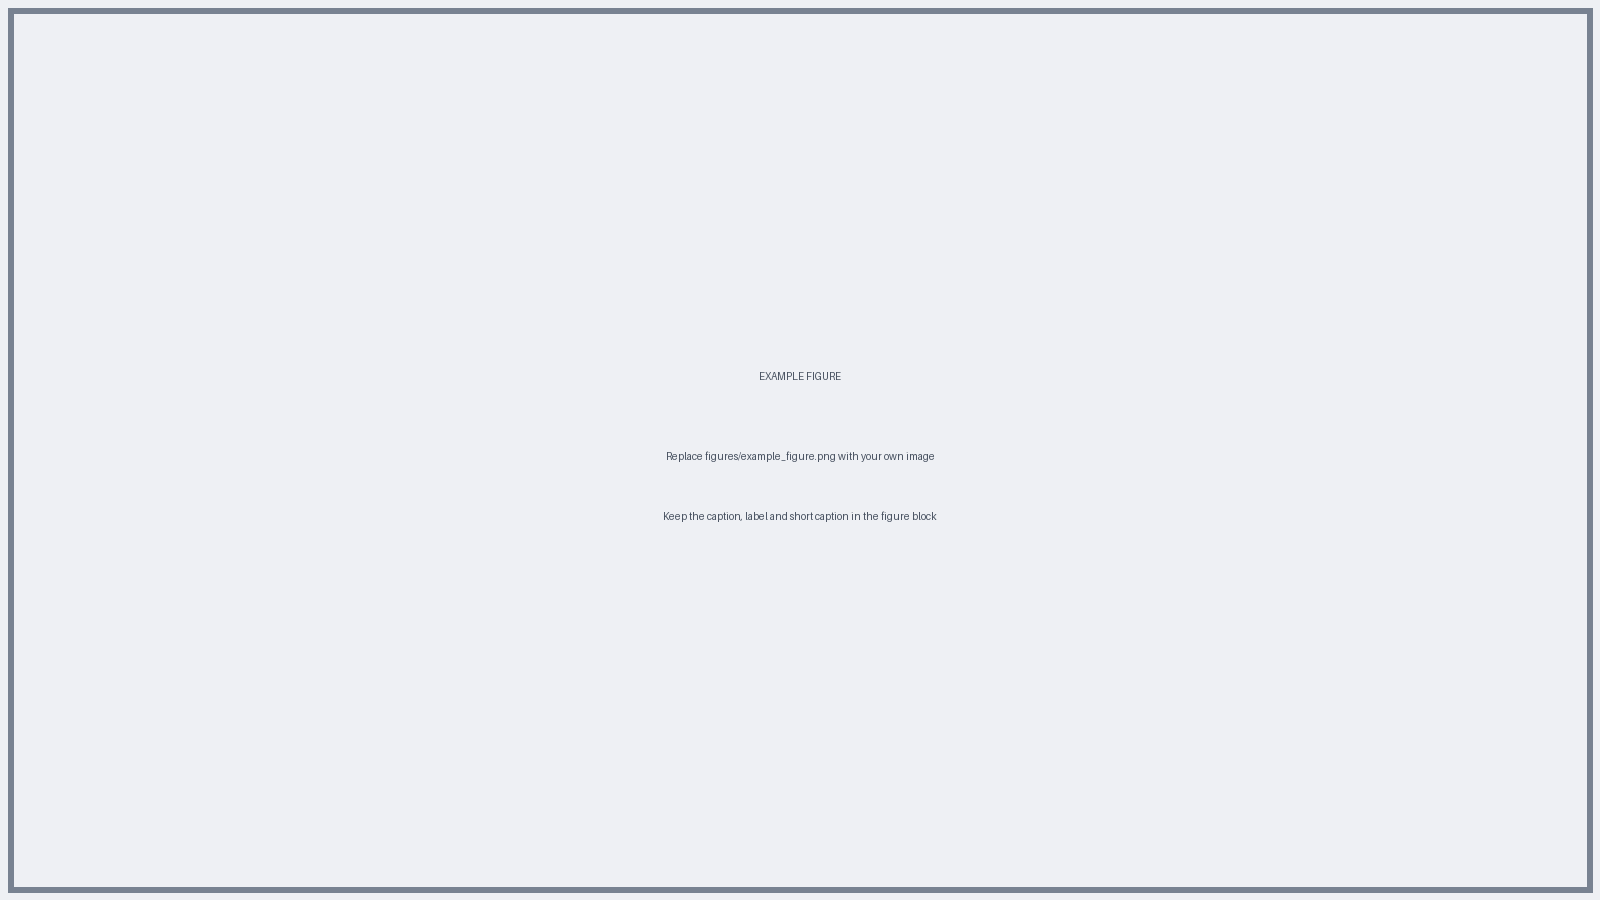
\includegraphics[width=0.85\textwidth]{figures/example_figure.png}
  \caption[Conceptual framework]{Conceptual framework linking [inputs], [evidence layers] and [the study outcome]. Source: author.}
  \label{fig:1.1}
\end{figure}

{[}Paragraph explaining the framework.]

\section{Research Scope}\label{sec:1.7}
\guidance{State what the study covers, where and when, and then state plainly what it does not cover. A clear boundary here prevents scope drift in Chapter 3 and protects you at the defence.}

{[}Scope: materials, sites, period, methods.]

{[}Boundary: this study will not \ldots]
